
The general equation of a plane is given by
\begin{align}
    px+qy+rz = c \label{eq:solutions/4/48/5/gen_plane_eqn}
\end{align}
and can be expressed as
\begin{align}
    \vec{n}^T\vec{x} = c \label{eq:solutions/4/48/5/plane_vec_eqn}
\end{align}
where
\begin{align}
    \vec{n} = \myvec{p \\ q \\ r}
\end{align}
The equation of a line passing through the point $a$ and having direction vector $\vec{b}$ is given by
\begin{align}
    \vec{x} = \vec{a} +\lambda \vec{b} \label{eq:solutions/4/48/5/vec_line_eq}
\end{align}
Rewriting given equation of plane in \eqref{eq:solutions/4/48/5/plane_vec_eqn} form, we get
\begin{align}\label{eq:solutions/4/48/5/eq0}
	\myvec{2 & -1 & 2}\myvec{x\\y\\z} = 5
\end{align}
where :
$\vec{n}=\myvec{2\\ -1 \\2}$, $\vec{x} = \myvec{x\\y\\z}$  and $c=5$\\
We need to represent equation of plane in parametric form,
\begin{equation}\label{eq:solutions/4/48/5/eq1}
	\vec{x} = \vec{p} + \lambda_1\vec{q} + \lambda_2\vec{r}
\end{equation}
Here $\vec{p}$ is any point on plane and $\vec{q}, \vec{r}$ are two vectors parallel to plane and hence $\perp$ to $\vec{n}$. Find two vectors that are $\perp$ to $\vec{n}$
\begin{align}\label{eq:solutions/4/48/5/eq2}
	\implies\myvec{2 & -1 & 2}\myvec{a\\b\\c} = 0
\end{align}
Put $a=1$ and $b=2$ in \eqref{eq:solutions/4/48/5/eq2}, $\implies c=0$\\
Put $a=0$ and $b=2$ in \eqref{eq:solutions/4/48/5/eq2}, $\implies c=1$\\
Hence $\vec{q} = \myvec{1\\2\\0}, \vec{r} = \myvec{0\\2\\1}$\\
Let us find point $\vec{p}$ on the plane. Put $x=1,y=-1$ in \eqref{eq:solutions/4/48/5/eq0}, we get $\vec{p} = \myvec{1\\-1\\1}$\\
Since given plane is perpendicular to given line, if we take $\vec{P} = \myvec{3 \\ 4 \\ -1}$ it will give us the shortest distance to the plane. \\
Let $\vec{Q}$ be the point on plane with shortest distance to $\vec{P}$. $\vec{Q}$ can be expressed in \eqref{eq:solutions/4/48/5/eq1} form as
\begin{align}\label{eq:solutions/4/48/5/eq3}
	\vec{Q} = \myvec{1\\-1\\1} + \lambda_1\myvec{1\\2\\0} + \lambda_2\myvec{0\\2\\1}
\end{align}
Equate $\vec{P}$ and $\vec{Q}$, and compute $\lambda_1, \lambda_2$ using $\textit{pseudoinverse}$ from $\textit{SVD}$
\begin{align}
	\myvec{1\\-1\\1} + \lambda_1\myvec{1\\2\\0} + \lambda_2\myvec{0\\2\\ 1} &= \myvec{3\\4\\-1}\\
	\lambda_1\myvec{1\\2\\0} + \lambda_2\myvec{0\\2\\ 1} &= \myvec{2\\5\\-2}\\
	\label{eq:solutions/4/48/5/eq4}\myvec{1 & 0\\2 & 2\\0 & 1} \myvec{\lambda_1 \\ \lambda_2} &=\myvec{2\\5\\-2}\\
	\label{eq:solutions/4/48/5/eq5}\vec{M}\vec{x} &= \vec{b}\\
	\label{eq:solutions/4/48/5/eq6}\implies\vec{x} &= \vec{M}^{+}\vec{b}
\end{align}
where $\vec{M} = \myvec{1 & 0\\2 & 2\\0 & 1}$, $\vec{x}= \myvec{\lambda_1 \\ \lambda_2}$ and $\vec{b}=\myvec{2\\5\\-2}$
Diagonalize $\vec{M}\vec{M}^T$
\begin{align}
	\vec{M}\vec{M}^T &= \myvec{1 & 0\\2 & 2\\0 & 1} \myvec{1 & 2 & 0\\0 & 2 & 1} = \myvec{1 & 2 & 0\\2 & 8 & 2\\ 0 & 2 & 1} 
\end{align}
We get three eigen values as 9, 1 and 0. Normalizing the eigen vectors, $\vec{U}$ is calculated as : 
\begin{align}
	\vec{U} &= \myvec{\frac{1}{3\sqrt{2}} & \frac{-1}{\sqrt{2}} & \frac{2}{3} \\ \frac{4}{3\sqrt{2}} & 0 & \frac{-1}{3} \\ \frac{1}{3\sqrt{2}} & \frac{1}{\sqrt{2}} & \frac{2}{3}}  
\end{align}
Diagonalize $\vec{M}^T\vec{M}$
\begin{align}
	\label{eq:solutions/4/48/5/e14}\vec{M}^T\vec{M} &= \myvec{1 & 2 & 0\\0 & 2 & 1}\myvec{1 & 0\\2 & 2\\0 & 1} = \myvec{5 & 4\\4 & 5}
\end{align}
We get two eigen values as 9, 1. Normalizing the eigen vectors, $\vec{V}$ is calculated as : 
\begin{align}
	\vec{V} &= \myvec{\frac{1}{\sqrt{2}} & \frac{-1}{\sqrt{2}} \\
	\frac{1}{\sqrt{2}} & \frac{-1}{\sqrt{2}}}  
\end{align}
Taking square root of eigen values, We get $\vec{\Sigma}$ as :
\begin{align}
	\vec{\Sigma} &= \myvec{3 & 0\\0 & 1\\0 & 0}
\end{align}
Thus, we performed Singular Value Decomposition for $\vec{M}$. It is easy to check that $\vec{U}\vec{\Sigma}\vec{V}^T = \vec{M}$. \\
For calculating the psuedoinverse, we know 
\begin{align}
\vec{M}^{+} &= \vec{V}\vec{\Sigma}^{-1}\vec{U}^T \\
&= \myvec{\frac{1}{\sqrt{2}} & \frac{-1}{\sqrt{2}} \\
	\frac{1}{\sqrt{2}} & \frac{-1}{\sqrt{2}}} \myvec{\frac{1}{3} & 0 & 0 \\ 0 & 1 & 0} \myvec{\frac{1}{3\sqrt{2}} & \frac{4}{3\sqrt{2}} & \frac{1}{3\sqrt{2}} \\ \frac{-1}{\sqrt{2}} & 0 &  \frac{1}{\sqrt{2}} \\  \frac{2}{3} & \frac{-1}{3} & \frac{2}{3}}\\
&= \label{eq:solutions/4/48/5/eq7}\myvec{\frac{5}{9} & \frac{2}{9} & \frac{-4}{9} \\ \frac{-4}{9} & \frac{2}{9} & \frac{5}{9}}
\end{align}

Substitute \eqref{eq:solutions/4/48/5/eq7} in \eqref{eq:solutions/4/48/5/eq6},
\begin{align}\label{eq:solutions/4/48/5/eq8}
	\vec{x} =\myvec{\frac{5}{9} & \frac{2}{9} & \frac{-4}{9} \\ \frac{-4}{9} & \frac{2}{9} & \frac{5}{9}}\myvec{2\\5\\-2} = \myvec{\frac{28}{9}\\\frac{-8}{9}} = \myvec{\lambda_1 \\ \lambda_2}
\end{align}
Substituting $\lambda_1$, $\lambda_2$ in \eqref{eq:solutions/4/48/5/eq3}
\begin{equation}
	\vec{Q} = \frac{1}{9}\myvec{37\\31\\1}
\end{equation}
Hence the equation of required line using \eqref{eq:solutions/4/48/5/vec_line_eq} is:
\begin{align}
     \vec{x} = \myvec{3\\4\\-1} +\lambda\myvec{2\\-1\\2} 
\end{align}
\begin{figure}[h]
    \centering
    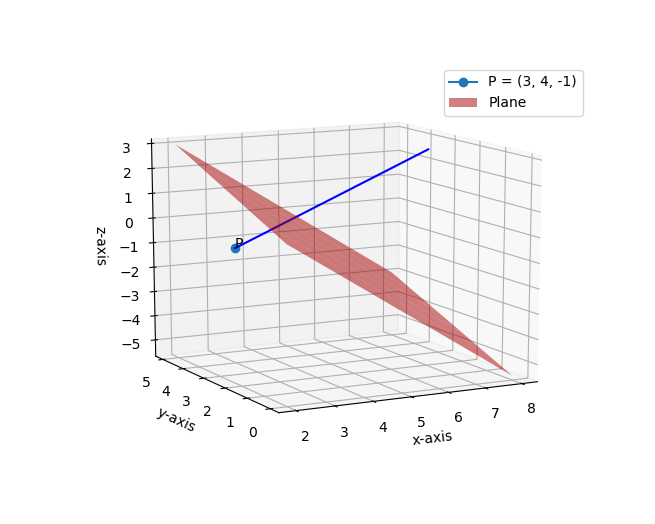
\includegraphics[width = \columnwidth]{./solutions/4/48/5/assignment_8.png}
    \caption{Line passing through $\myvec{3 & 4 & -1}$ and perpendicular to the plane $2x - y + 2z = 5$.}
    \label{eq:solutions/4/48/5/line and plane}
\end{figure}
\newpage
Verifying solution to \eqref{eq:solutions/4/48/5/eq5} with $\textit{least squares}$ method
\begin{align}
	\vec{M}^T(\vec{b} - \vec{M}\vec{x}) &= 0\\
	\label{eq:solutions/4/48/5/eq9}\implies \vec{M}^T\vec{M}\vec{x} &= \vec{M}^T\vec{b}
\end{align}
Substituting $\vec{M}, \vec{b}$ from \eqref{eq:solutions/4/48/5/eq4} in \eqref{eq:solutions/4/48/5/eq9}
\begin{align}
	\myvec{1 & 2 & 0\\0 & 2 & 1}\myvec{1 & 0\\2 & 2\\0 & 1}\vec{x} &= \myvec{1 & 2 & 0\\0 & 2 & 1}\myvec{2\\5\\-2}\\
	\myvec{5 & 4\\4 & 5}\myvec{\lambda_1\\\lambda_2} &= \myvec{12\\8}\\
	\implies5\lambda_1 + 4\lambda_2&= 12\\
	4\lambda_1 + 5\lambda_2&= 8\\
	\lambda_1 &= \frac{28}{9}\\
	\text{and }\lambda_2 &= \frac{-8}{9}\\
	\label{eq:solutions/4/48/5/eq10}\implies\vec{x} &= \myvec{\frac{28}{9}\\\frac{-8}{9}}
\end{align}
Comparing \eqref{eq:solutions/4/48/5/eq8} and \eqref{eq:solutions/4/48/5/eq10} solution is verified.
